\section{Aktive Filter}

\subsection{Filter 1. Ordnung}

\subsubsection{Integrator}
\begin{multicols}{2}
	\begin{center}
		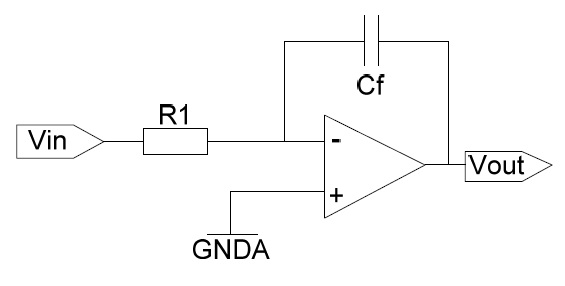
\includegraphics[width=6cm]{images/filter_1_integrator.jpg}
	\end{center}
	\begin{align*}
		T(s) &= Y_{\In} \Zop = - \frac{1}{s C_f R_1} \\
		V_{\Out} &= -\frac{1}{R_1 C_f} \int V_{\In} dt + V_0
	\end{align*}
\end{multicols}

\subsubsection{Tiefpass}
\begin{multicols}{2}
	\begin{center}
		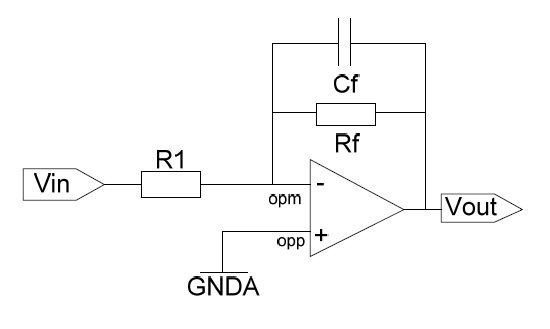
\includegraphics[width=6cm]{images/filter_1_tiefpass.jpg}
	\end{center}
	\begin{align*}
		T(s) &= -\frac{R_f}{R_1} \cdot \frac{1}{1 + s C_f R_f}
	\end{align*}
\end{multicols}

\newpage
\subsubsection{Differenzierer}
\begin{multicols}{2}


	Achtung: dieser Differenzierer schwingt meistens.
	\begin{center}
		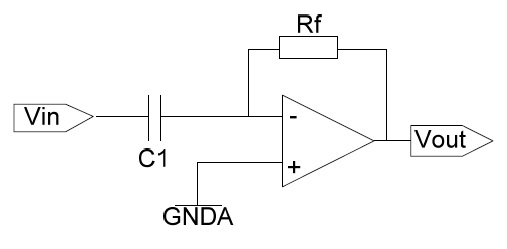
\includegraphics[width=6cm]{images/filter_1_diff.jpg}
	\end{center}
	\begin{align*}
		T(s) = -s C_1 R_f
	\end{align*}
\vfill	
\columnbreak
	Bandpass mit differenzierendem Frequenzbereich
	\begin{center}
		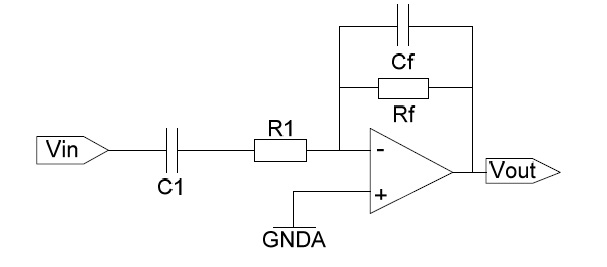
\includegraphics[width=0.7\linewidth]{images/filter_1_diff2.jpg}
	\end{center}
	\begin{align*}
		T(s) = - \frac{s C_1 R_f}{1 + s C_1 R_1} \cdot \frac{1}{1 + s C_f R_f}
	\end{align*}
	Differenziert zwischen $\omega_1 = \frac{1}{R_1 C_1}$ und 
	$\omega_2 = \frac{1}{R_f C_f}$

\end{multicols}

\subsection{Filter höherer Ordnung}

\begin{multicols}{2}
	\paragraph{Tiefpass 2. Ordnung}
	\begin{equation*}
		T_{TP}(s) = \frac{A \omega_0^2}{s^2 + \frac{\omega_0}{Q} s + \omega_0^2}
	\end{equation*}
	
	\paragraph{Bandpass 2. Ordnung}
	\begin{equation*}
		T_{BP}(s) = \frac{A \frac{\omega_0}{Q} s}{s^2 + \frac{\omega_0}{Q} s + \omega_0^2}
	\end{equation*}
\end{multicols}


\subsubsection{Sallen-Key Filter}
\paragraph{Sallen-Key Tiefpass}
\begin{center}
	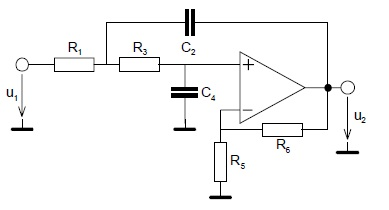
\includegraphics[width=8cm]{images/filter_sk_tp.jpg}
\end{center}
\begin{equation*}
	T(s) = \frac{A}{1 + \left(R_3 C_4 + R_1 C_4 + R_1 C_2 (1-A)\right) \cdot s + R_1 R_3 C_2 C_4 \cdot s^2}
\end{equation*}

\paragraph{Sallen-Key Bandpass}
\begin{center}
	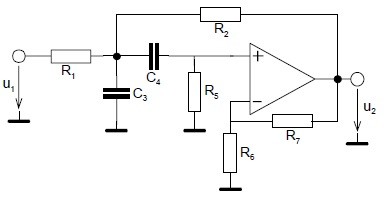
\includegraphics[width=8cm]{images/filter_sk_bp.jpg}
\end{center}
\begin{equation*}
	T(s) = \frac{\frac{R_2 R_5}{R_1 + R_2} C_4 A_M \cdot s}{1 + \frac{R_1 R_5 C_4 (1-A_M) + R_1 R_2 (C_3 + C_4) + R_2 R_5 C_4}{R_1 + R_2} \cdot s + \frac{R_1 R_2}{R_1 + R_2} R_5 C_3 C_4 \cdot s^2}
\end{equation*}
mit $A_M = 1+\frac{R_7}{R_6}$

\subsubsection{Multiple Feedback Filter}
\begin{center}
	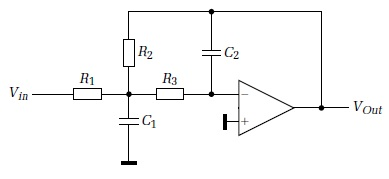
\includegraphics[width=8cm]{images/filter_mfb.jpg}
\end{center}
\begin{align*}
	T(s) &= \frac{G_0}{1 + C_s \left(R_2 + R_3 + R_3 \frac{R_2}{R_1}\right) \cdot s + C_1 C_2 R_2 R_3 \cdot s^2} \qquad \text{mit} \quad G_0 = -\frac{R_2}{R_1} \\
	Q &= \frac{\sqrt{C_1 C_2 R_2 R_3}}{C_2 \left(R_2 R_3 R_3 \frac{R_2}{R_1}\right)}
\end{align*}
Die Güte wird v.a. mit $C_2$ und $R_1$ eingestellt.


\subsection{Biquads}
Beispiel Bandpass:
\begin{center}
	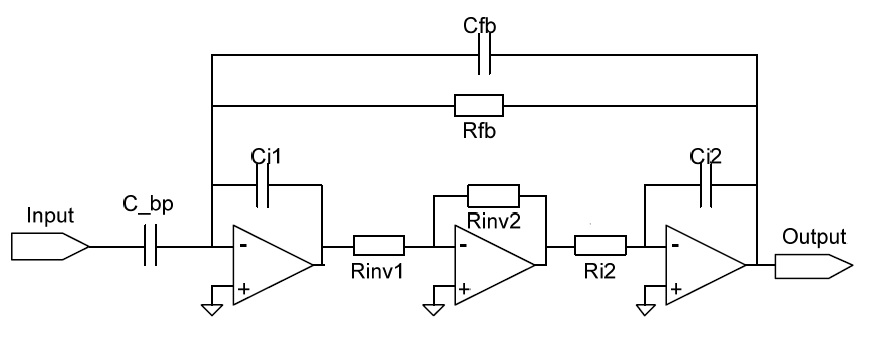
\includegraphics[width=8cm]{images/filter_biquad.jpg} 
	\hspace{2cm}
	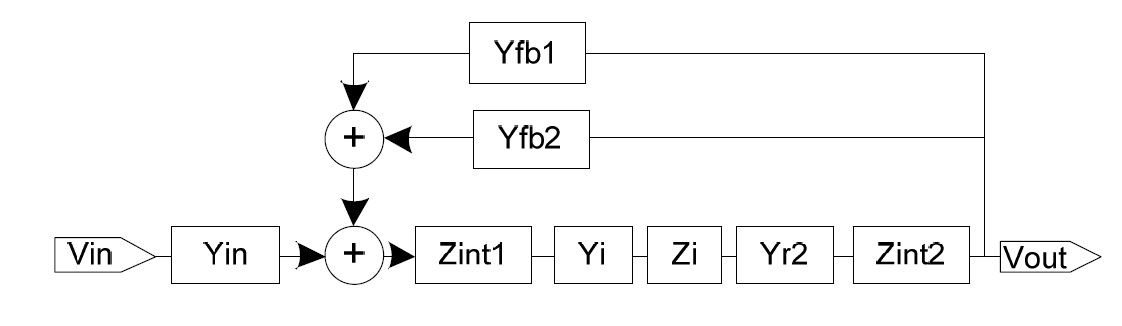
\includegraphics[width=8cm]{images/filter_biquad_block.jpg} 
\end{center}
\begin{align*}
	T(s) &= \frac{Y_{\In} Z_{\Int 1} Y_i Z_i Y_{r 2} Z_{\Int 2}}{1 - (Y_{\Fb 1}+Y_{\Fb 2}) Z_{\Int 1} Y_i Z_i Y_{r 2} Z_{\Int 2}}
	&= \frac{\frac{C_{bp}}{C_{i1} R_{i2} C_{i2}} \cdot s}{s^2 + \frac{C_{fb}}{C_{i1} R_{i2} C_{i2}} \cdot s + \frac{1}{R_{fb} C_{i1} R_{i2} C_{i2}}}
\end{align*}
und damit
\begin{equation*}
	A = -\frac{C_{bp}}{C_{fb}} \qquad Q = \sqrt{\frac{R_{i2}}{R_{fb}}} \cdot \frac{\sqrt{C_{i1} C_{i2}}}{C_{fb}} \qquad f_0 = \frac{1}{2 \pi \sqrt{C_{i1} C_{i2} R_{fb} R_{i2}}}
\end{equation*}

%TODO: Tiefpass, Abgeänderte Version, Tow Thomas, Ackerberg-Mossberg